%==============================================================================
% Figure: Quaternion Multiplication via Fano Plane
% Purpose: Visualize octonion multiplication rules using Fano plane geometry
% Chapter: Ch02 - Cayley-Dickson Algebras
% Type: Mathematical
%==============================================================================

\begin{figure}[htbp]
  \centering
  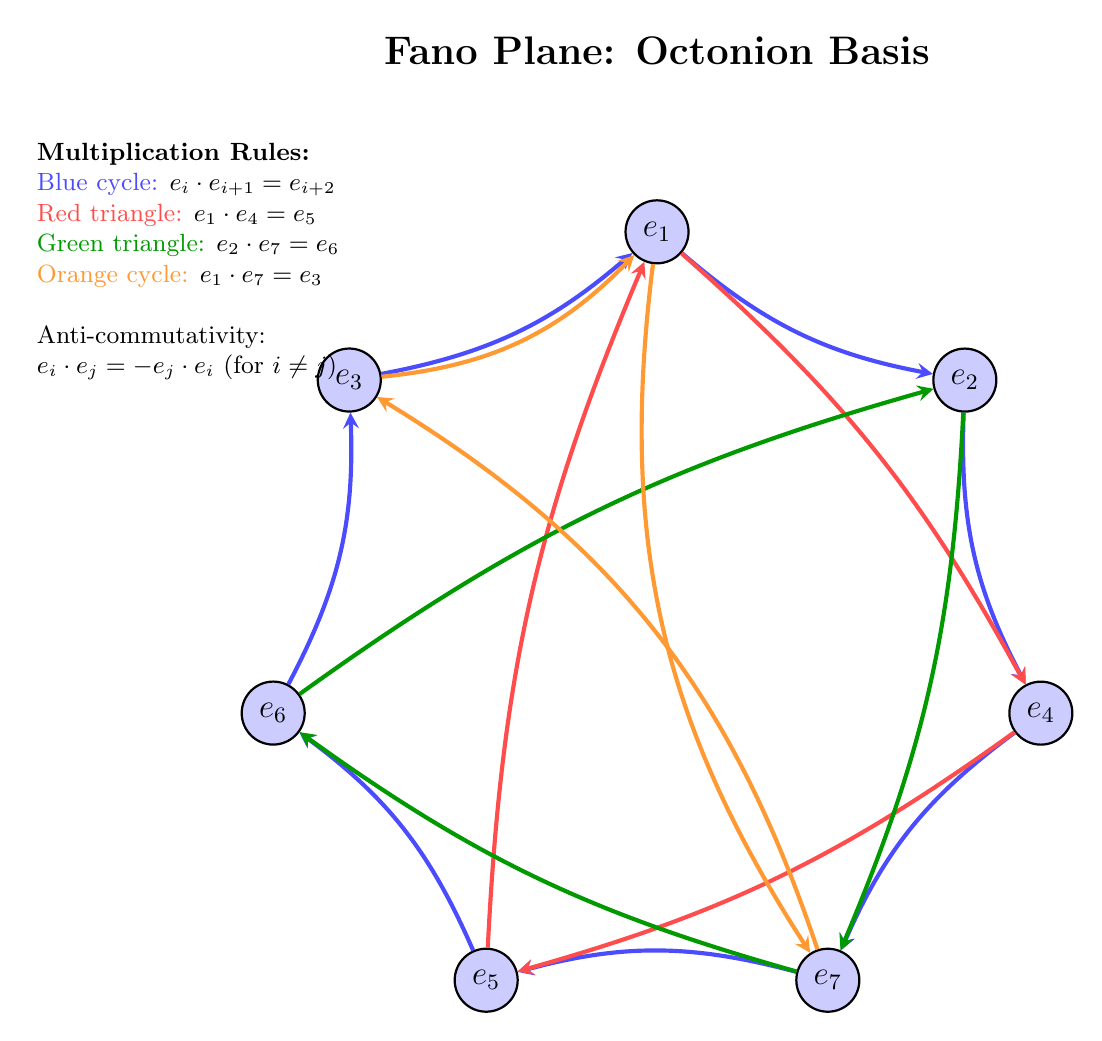
\begin{tikzpicture}[
    scale=2.5,
    vertex/.style={circle, draw=black, fill=blue!20, thick, minimum size=8mm},
    edge/.style={->, thick, >=stealth},
    label/.style={font=\large\bfseries}
  ]

    % Define the 7 vertices of the Fano plane in a circular arrangement
    \def\radius{2}
    \foreach \i/\label in {0/e_1, 1/e_2, 2/e_4, 3/e_7, 4/e_5, 5/e_6, 6/e_3} {
      \pgfmathsetmacro\angle{90 - \i * 51.43}  % 360/7 = 51.43 degrees
      \node[vertex, label] (v\i) at (\angle:\radius) {$\label$};
    }

    % Draw the outer circle (connecting consecutive vertices)
    % Cycle: e1 -> e2 -> e4 -> e7 -> e5 -> e6 -> e3 -> e1
    \foreach \i [evaluate=\i as \next using {int(mod(\i+1, 7))}] in {0,...,6} {
      \draw[edge, blue!70, line width=1.5pt] (v\i) to[bend right=15] (v\next);
    }

    % Draw the inner triangle lines
    % Triangle 1: e1 -> e4 -> e5 -> e1 (vertices 0, 2, 4)
    \draw[edge, red!70, line width=1.5pt] (v0) to[bend left=10] (v2);
    \draw[edge, red!70, line width=1.5pt] (v2) to[bend left=10] (v4);
    \draw[edge, red!70, line width=1.5pt] (v4) to[bend left=10] (v0);

    % Triangle 2: e2 -> e7 -> e6 -> e2 (vertices 1, 3, 5)
    \draw[edge, green!60!black, line width=1.5pt] (v1) to[bend left=10] (v3);
    \draw[edge, green!60!black, line width=1.5pt] (v3) to[bend left=10] (v5);
    \draw[edge, green!60!black, line width=1.5pt] (v5) to[bend left=10] (v1);

    % Central inscribed circle (connecting alternating vertices)
    \draw[edge, orange!80, line width=1.5pt] (v0) to[bend right=20] (v3);
    \draw[edge, orange!80, line width=1.5pt] (v3) to[bend right=20] (v6);
    \draw[edge, orange!80, line width=1.5pt] (v6) to[bend right=20] (v0);

    % Legend showing multiplication rules
    \node[anchor=north west, align=left, font=\small] at (-3.2, 2.5) {
      \textbf{Multiplication Rules:} \\
      \textcolor{blue!70}{Blue cycle:} $e_i \cdot e_{i+1} = e_{i+2}$ \\
      \textcolor{red!70}{Red triangle:} $e_1 \cdot e_4 = e_5$ \\
      \textcolor{green!60!black}{Green triangle:} $e_2 \cdot e_7 = e_6$ \\
      \textcolor{orange!80}{Orange cycle:} $e_1 \cdot e_7 = e_3$ \\
      \\
      Anti-commutativity: \\
      $e_i \cdot e_j = -e_j \cdot e_i$ (for $i \neq j$)
    };

    % Title annotation
    \node[anchor=south, font=\Large\bfseries] at (0, 2.8) {Fano Plane: Octonion Basis};

  \end{tikzpicture}
  \caption{Quaternion and octonion multiplication structure visualized via the Fano plane.
    The 7 imaginary units ($e_1$ through $e_7$) form vertices, with oriented lines showing
    multiplication paths. Following any oriented line from $e_i$ to $e_j$ gives $e_i \cdot e_j = e_k$
    where $e_k$ is the third vertex on that line. Reversing the direction introduces a minus sign
    due to anti-commutativity. The color-coded cycles represent different multiplication families
    within the octonion algebra \textbf{O}. This structure encodes the non-associative nature
    of octonions while maintaining alternativity.}
  \label{fig:quaternion-multiplication}
\end{figure}
